\documentclass{article}
\usepackage[T1]{fontenc}
\usepackage[utf8]{inputenc}
\usepackage[margin=1in]{geometry}
\usepackage{amsmath}
\usepackage{graphicx}

\newcommand{\HRule}{\rule{\linewidth}{0.5mm}}
\newcommand{\Hrule}{\rule{\linewidth}{0.3mm}}

\title{Lab Report 1}
\author{Yuhuang Chen (804449266), Zeyuan Xu (004255573)}
\date{}
\begin{document}
  \maketitle% prints the title block
  \thispagestyle{empty}

\section{Part 1: 1 Bit ALU}
\subsection{Introduction}
\begin{figure}[h]
  \centering
  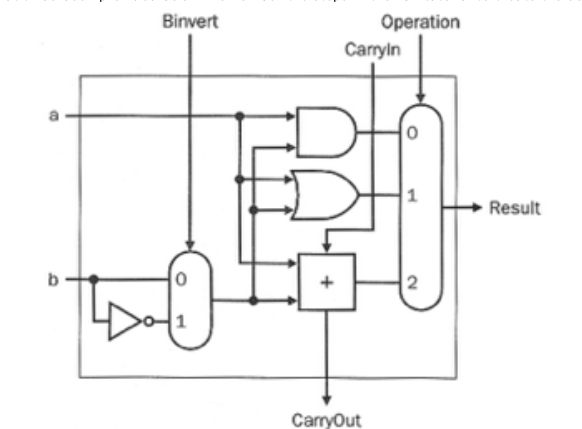
\includegraphics[width=\linewidth]{1-Bit-ALU.png}
  \caption{1-Bit-ALU}
  \label{fig:1-ALU}
\end{figure}
In the first part, we simply need to follow the diagram (figure 1) to implement an 1-bit ALU, which has components as: OR gate, AND gate, NOT gate, 1-bit full adder, 2-1 mux, and 3-1 mux. The 2-1 mux is easily implemented via the logical gate specified in figure 2. The 4-1 mux is simply hooked up in the logic specified in figure 3. 
The schematic diagram is: 
\begin{figure}[!htb]
\minipage{0.5\textwidth}
  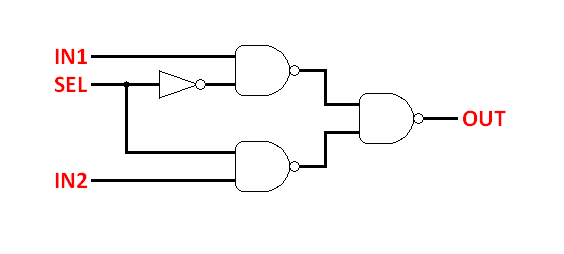
\includegraphics[width=\linewidth]{mux2-1.png}
  \caption{2-1 mux}\label{fig:mux2-1}
\endminipage\hfill
\minipage{0.5\textwidth}
  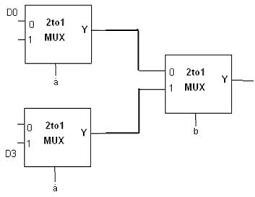
\includegraphics[width=\linewidth]{mux4-1.png}
  \caption{4-1 mux}\label{fig:mux4-1}
\endminipage\hfill
\end{figure}

\subsection{Simulation Result}
The simulation result for the 1-bit ALU is shown in figure 4, in which all operations are tested and verified. 
\begin{figure}[h]
  \centering
  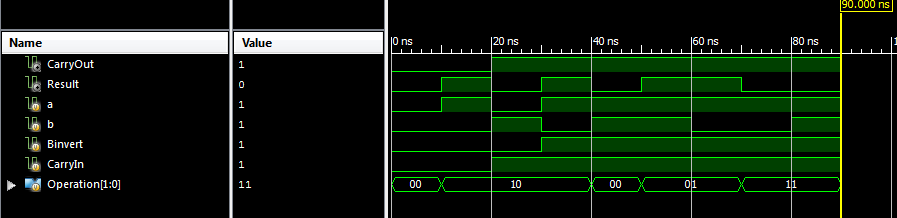
\includegraphics[width=\linewidth]{lab1-1.PNG}
  \caption{1-bit ALU demo}
  \label{fig:1-ALU}
\end{figure}
\subsection{Discussion}
Nothing particular is notieable about the 1-bit ALU. It sets the logic for further implementation of 16 bit ALU, whose structural builds upon it. 

\section{Part 2: 16 Bit ALU}
\subsection{Introduction}
The 16-bit ALU consists consists of operations specified in figure 5. The most complicated part of the ALU design is to design the 16 bit full adder, which should also contain overflow detection. The 16-1 mux is built upon by 4-1 mux, and the logic is depicted in figure 6. The 16-1 mux is shown in figure 7. The adder is implemented as a ripple adder. When buiding the 16-bit adder, we first build 4-bit adder from 1-bit adders, then using the same method to construct the 16-bit adder from the 4-bit adders. The logic can be depicted in figure 8. 
\begin{figure}[h]
  \centering
  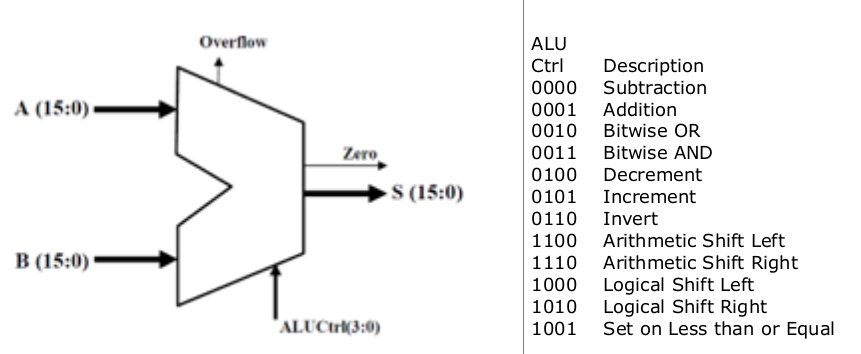
\includegraphics[width=\linewidth]{16-alu.png}
  \caption{16-bit ALU}
  \label{fig:16-ALU}
\end{figure}


\begin{figure}[!htb]
\minipage{0.33\textwidth}
  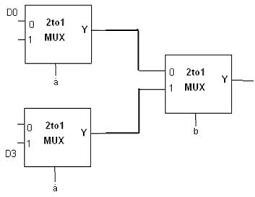
\includegraphics[width=\linewidth]{mux4-1.png}
  \caption{4-1 mux}\label{fig:mux4-1}
\endminipage\hfill
\minipage{0.33\textwidth}
  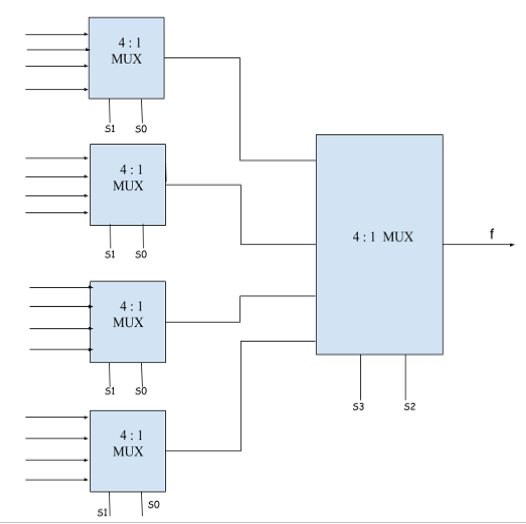
\includegraphics[width=\linewidth]{mux16-1.png}
  \caption{16-1 mux}\label{fig:mux16-1}
\endminipage\hfill
\minipage{0.33\textwidth}
  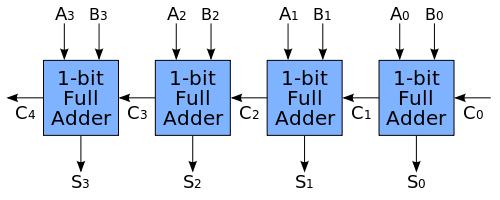
\includegraphics[width=\linewidth]{4-adder.png}
  \caption{4 bit adder}\label{fig:4-adder}
\endminipage\hfill
\end{figure}


\subsection{Simulation Result}

The simulation result is in figure 9.
\begin{figure}[!htb]
  \centering
  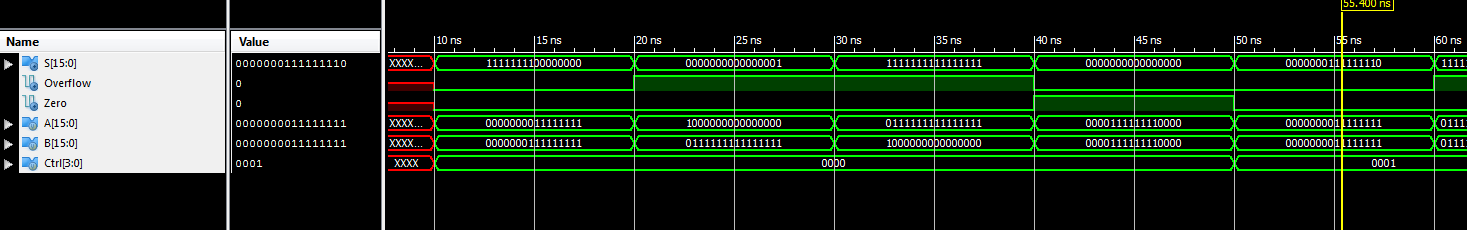
\includegraphics[width=\linewidth]{lab1-2.PNG}
  \caption{16-bit ALU demo}
  \label{fig:16-ALU demo}
\end{figure}



\subsection{Discussion}
The difficulties encountered for the 16-bit ALU design are: 
1. The overflow handling: the logic is that when two positive numbers add, and the result's sign bit is 1, have an overflow. This generic case is complicated by: in the subtraction case, when a positive number subtract a negative number, but result is negative, or a negative number minus a positive number, but result is positive. When we implement the set less than operation, we also need to specify the logic: 
\begin{verbatim}
logic here
\end{verbatim}


\section{Part 3: Register File }
\subsection{Introduction}

\subsection{Simulation Result}

\subsection{Discussion}



\section{Part 4: Questions and Answers}


\end{document}